\documentclass{article}
\usepackage[utf8]{inputenc}
\usepackage[margin=1in]{geometry}
\usepackage{graphicx}
\usepackage{natbib}
\usepackage{enumitem}
\usepackage{array}
\usepackage{gensymb}
\usepackage{indentfirst}
\graphicspath{ {Images/} }
\usepackage{float}
\usepackage[table,xcdraw]{xcolor}

\title{Physics 111A Fall 2016- Lab 4\\
JFET Circuits I}
\author{Joshua Levy\\Lab Partner: Alex Chuang}
\date{September 23rd, 2016}

\begin{document}

\maketitle

\section{Lab Writeup}
\subsection{Basic JFET Checks}
    DMM diode tests across various transistor components yielded:\\
    \indent $V_{SG} = $ "OPEN"\\
    \indent $V_{DG} = $ "OPEN"\\
    \indent $V_{DS} = $ 0.04V\\
    \indent $V_{GD} = $ 0.759V\\
    \indent $V_{GS} = $ 0.7605V\\
    \indent $V_{SD} = $ 0.04V\\
    The "OPEN" measurements between drain and gate and the source and gate are indicative of reverse biasing for the setup, which means that our transistor is working and ready for use. We also see that voltage drops between source and drain are the same either way.

\subsection{JFET Switch}
    The resistor, $R_{1}$ we placed in the circuit that was meant to be 1k measured: $R_{1} = 1.04k$, and the resistor $R_{22}$, meant to have a resistance of 22M, measured 17.8M. After placing $R_{22}$ into the circuit, we could still switch on the LED.

\subsection{JFET Memory}
    The "memory time" of the circuit without an external capacitor ($C_{add}$) being added was: $T_{w/oCadd} = 46.40s$. \\\indent With $C_{add}$ hooked up in parallel to the transistor gate  (thereby increasing the equivalent capacitance between the internal capacitance of the transistor gate and $C_{add}$; $C_{eq} = C_{add} + C_{iss}$), the "memory" time rose to 153 seconds. \\\indent The measured $C_{add} = 24.2 pF$. This capacitance was used because a 100pF capacitor yielded far too high of a memory time and was taking too long for us to finish our measurement.

\subsection{JFET Gate Transfer Characteristic}
    See signature page.
    
\subsection{JFET Gate Transfer Characteristic: Curve Tracer}
    Figure 1 depicts the transfer characteristic curve of the JFET gate. The data points added to the figure can be found in table 1. \\ Using our data, for a $V_{GS}$ of about -1V, and taking a direct differentiation of our data set, we find that $g_m \approx 1.41*10^{-2} [1/\Omega]$ and $r_s = \frac{1}{g_m} \approx 71.1 \Omega$. Unfortunately, the curve tracer we were using was malfunctioning, and gave us NaN values for all transconductance and internal resistance values. So a curve (parabola) was fit to data above a $V_{GS}$ value of -2.6V, yielding the equation:\\
    \begin{equation}
        i_d(V_{GS}) = 0.0025V_{GS}^{2} + 0.0191V_{GS} + 0.0324
    \end{equation}
    with an $R^{2}$ value of $99.8\%$, indicating that the data is a very nice fit over the range $V_{GS}\in [-2.6V,0]$. Direct differentiation of this equation yields:
    \begin{equation}
        g_m(V_{GS}) = 0.005V_{GS} + 0.0191
    \end{equation}
    $r_s$ is correspondingly:
    \begin{equation}
        r_s(V_{GS}) = \frac{1}{0.005V_{GS} + 0.0191}
    \end{equation}
    The range is limited in these two instances to $V_{GS}\in [-2.6V,0]$, because at values lower than $V_{GS} = 2.6V$, the current flattens out and a parabola is no longer able to fit the data. The linear and saturated regimes of the JFET output curve have been plotted in figure 2.

\subsection{JFET Gate Transfer Characteristic: Curve Tracer for the 2N3819}
    See Figure 3 for a plot of the 2N3819 JFET Transfer Curve and for a plot of the Transconductance vs $V_{GS}$. It would appear that a parabola is a good fit for the data for $V_{GS}\in [-2.2V,0]$. The transconductance data plotted in this range appears to form a nice linear fit, with \begin{equation}
        g_m(V_{GS}) = 0.0026V_{GS} + 0.0058
    \end{equation}
    and an $R^{2}$ value of 96.7 $\%$. The plot of the characteristic output curve over that range exemplifies a nice parabola-fit. 
    

\subsection{JFET Thermal Properties}
    The 1 mA current does not drift a lot. It drifts far less than the the 15 mA current. The 1 mA current does not drift a lot because there is less power being dissipated across the transistor, so the transistor does not heat up, so it experiences not a lot of increase in internal resistance. As you increase the current, more power is dissipated, increasing internal resistance as the transistor heats up, thus decreasing the current over time. We model the power being dissipated across the transistor by first finding the voltage drop across the transistor:
    \begin{equation}
        V_{DS} = 12V - i*R
    \end{equation}
    Where the current is i, and R (100$\Omega$) was measured to be 102 $\Omega$, and 12V is our power supply. The power dissipated is:
    \begin{equation}
        P_{DS} = i*V_{DS} = i*12V - i^{2}R
    \end{equation}
    Plugging in i = 1 mA, and $P_{DS} \approx 0.0119W$. Plugging in i = 15 mA, and $P_{DS} \approx 0.1571W$. The transistor gets much hotter with a current of 15 mA, and spraying the cooler on the JFET counters the drift and increases the current towards 15 mA and higher because the cooling will decrease internal resistance thereby increasing current.

\subsection{JFET Self Biased Current Source}
    See signature page.
    
\subsection{Adjustable Self Biased Current Source}
    In [4.8], we used a resistor of value $703 \Omega$, and for a total Voltage across the JFET and resistor ($V_{DG}$) of 15 V, we measured a current of $\sim$ 2.96 mA. In this section, we measured the current for resistor values of 100$\Omega$, 390$\Omega$, 3.3k$\Omega$, and 10k$\Omega$. However, for the 100$\Omega$ and 390$\Omega$ resistors, measured 103.6$\Omega$ and 386.9$\Omega$ respectively, current values were omitted from the analysis, because at such low resistor values, the current approached its current limit of 24 mA, which thereby current-limited the input voltage. This would yield unreliable data. The rest of the results can be found on table 2. \\\indent Load line analyses were done on the data to predict output currents, where the load line:
    \begin{equation}
        I_D (V_{GS}) = -\frac{V_{GS}}{R}
    \end{equation}
    is intersected with the curve found in [4.5] (figure 1) for given resistance values. This intersection was found via graphical analysis, which is portrayed in figure 4, with results included in table 2. Looking at the results from table 2, we see that there is very low relative error between the measured current and the current predicted from loadline analysis, with error values below 6$\%$. This suggests that our measured current values agree with the predicted current values.

\subsection{JFET Source-Drain Output Characteristics: Externally Biased Current Source}
    Having burned out a few JFETs at this point from forward biasing the gate voltage, the plots for the characteristic curves for the new transistor can be found in Figure 5, and from here forth, data will be used from this new JFET. Looking at Figure 5, the data appears to be more reliable in this case, and appears to match with expectations of how a JFET curve should be.\\\indent Holding the voltage from the signal generator at -3V, the voltage dropped across the JFET $V_{DS}$ and measured current $i_d$ have been measured and plotted between table 3 and figure 6. The current for $V_{ds}$ of 15 V is 2.94 mA. After spraying the circuit cooler, this current increases to 2.97 mA. $I_D$ increases by 0.03 mA.

\subsection{Comparing Current Sources}
    In the previous section, the current was plotted as a function of $V_{DS}$ (figure 6) for the externally biased current source. For the self-biased current source of [4.8] (Table 6), the data has been plotted in figure 7. A linear fit was found for each plot for larger $V_{drop}$ voltage drop values (these data points look appropriately linear), and the stiffness was found by taking the inverse of the slope of such a fit.\\\indent For the self-biased current source, this stiffness was calculated to be $\approx  200000\Omega$  \\\indent For the externally biased current source, this stiffness was calculated to be $\approx 50000\Omega$. This stiffness of the self-biased current source is about four times larger than the stiffness of the externally biased current source. 
    
\subsection{Source Followers}
    See signature page.
    
\subsection{Source Follower Gain}
    The gain G, is:
    \begin{equation}
        G = \frac{V_{out}}{V_{in}} \approx 1 + \frac{\Delta V}{V_{in}}
    \end{equation}
    where:
    \begin{equation}
        \Delta V = V_{out} - V_{in}
    \end{equation}
    For a $V_{in} = 304 mV$ and $V_{out} = 280 mV$, the gain is calculated to be 
    \begin{equation}
        G = 1 + \frac{280 - 304}{304} \approx 0.921
    \end{equation}
    The predicted Gain of the circuit is found by:
    \begin{equation}
        G_p = \frac{V_{out}}{V_{in}} = \frac{R_s}{R_s + r_s}
    \end{equation}
    where $R_s$ is the resistor in series with the JFET and $r_s$ is the internal resistance of the transistor. Because we are using a new JFET, we calculate a new parabolic curve to fit the transfer curve.\\\indent
    Choosing reasonable data points for $V_{GS}\in[-2.7V,0V]$, and we find fir the curve:
    \begin{equation}
        i_d(V_{GS}) = 0.0025V_{GS}^{2} + 0.0193V_{GS} + 0.0332
    \end{equation}
    with $R_{2}$ of 99.8$\%$ (really good fit). Differentiating and taking the inverse, and we find that in that region:
    \begin{equation}
        r_s = \frac{1}{0.005 V_{GS} + 0.0193} \Omega
    \end{equation}
    $V_{GS}$ can be found through small signal analysis, by assuming $V_{GS} \approx 0$ (because the signal oscillates about 0V), and plugging this into eq.13 yields $r_s \approx 51.8 \Omega$. $R_s$ was measured to be $341 \Omega$. So
    \begin{equation}
        G_p = \frac{341}{51.8 + 341} \approx 0.868
    \end{equation}
    Our measured gain was $\sim 0.921$ whereas our predicted gain was $\sim 0.868$, leading us to a relative error of:
    \begin{equation}
        Err_{relative} = |\frac{G_{meas} - G_p}{G_p}| = \frac{0.921 - 0.868}{0.868} \approx 0.0601\%
    \end{equation}
    This amount of error is very reasonable. Anything over 10 percent error would not be in as much agreement, and thus, assuming a small signal, we have agreement between the measured and predicted value.
    
\subsection{Problem 4.14}
    As we modified the potentiometer ($R_L$), we noticed that decreasing $R_L$ decreases our output voltage. We were told that when $V_{out} = \frac{V_{in}}{2}$, the output impedance Z of the follower will equal $R_L$. We found that this occurs when $R_L \approx 0.9 \% * 10k = 90 \Omega$. We used an $R_s$ value of 330$\Omega$. From this, and using the equation given in this problem in the lab handout:
    \begin{equation}
        Z_{out} = \frac{r_s R_s}{r_s + R_s}
    \end{equation}
    We find, after some rearrangement, that 
    \begin{equation}
        r_s = \frac{R_s Z}{R + Z} = \frac{330 \Omega * 90 \Omega}{(330 + 90)\Omega} \approx 70.7 \Omega
    \end{equation}
    Leading us to find a transconductance of
    \begin{equation}
        g_m = \frac{1}{r_s} = \frac{1}{70.7 \Omega} \approx 0.01414 [\frac{1}{\Omega}]
    \end{equation}

\subsection{Matching JFETs}
    We grabbed five different JFETs and measured the currents of each of them for a given $R = 339\Omega$. See table 4 for the results of all of the JFETs. The third JFET measured a current of 5.49 mA, which was the closest to the original JFET's measurement and within the 10$\%$ threshold. We use this JFET to construct the improved follower.
    
\subsection{Improved Follower I}
    Table 5 compares the input and output for a variety of input signals, and displays the measured gain of each system. The measured gain was calculated using eq.(9). These measured gain values are quite large ($\textgreater$0.95$\%$), so we are not seeing a lot of discernible difference between the output and input amplitudes.\\\indent 
    In [4.11], the stiffness was calculated to be $\approx  200000\Omega$. We set this to be $R_s$. We utilize eq.(13) for internal resistance $r_s$, and since the signal $V_{in}$ oscillates about 0V, we can assume a small signal resistance model. \\\indent However, the current $i_d$ passing through the circuit corresponds to self-biased current source that is in series with the follower. The current source puts out a constant current, so $V_{GS}$ is found by intersecting the characteristic curve of the diode with the constant line $i_d$ = 0.00294 A (as determined by the interpolation of data between 10V and 15V voltage drop from Table 6, if we assume our circuit is now a self-biased current source in series with a 12V power supply, a JFET and resistor $R_s$). We find $V_{GS}$ to be $\approx$ -2.13 V after interpolating the transfer curve data to find the $V_{GS}$ that corresponds to $i_d$ = 0.00294 A.\\\indent  Using eq.13, and the $V_{GS}$ found,
     we find the corresponding $r_s$ calculated (using eq.(13)) values in Table 7. The predicted gain for each of the $V_{in}$, corresponding $r_s$ value ($\sim 116\Omega$), and stiffness of $200000\Omega$ (now set to $R_s$) is found using eq.(11), and is output to Table 7. Regardless, the Gain $G = \frac{200000\Omega}{200000\Omega + 115\Omega} \approx 0.9994$.  Relative Errors (eq.15) have also been computed for each gain value.\\\indent 
     The relative error between the predicted and measured gains are insignificant ($\textless$5$\%$ error), and the high stiffness of $R_s$ from the self-biased current source has led to major increases in gain and an output signal nearly equal to the input signal. Observed and expected values seem to agree.
    

\subsection{Improved Follower II}
    See signature page.
    
\subsection{Follower Feedback}
    Maintaining the follower's linearity would require a gain that maintains the proportionality between $V_{out}$ and $V_{in}$. We note that our gain is
    \begin{equation}
        G = \frac{R_s}{R_s + r_s} = \frac{R_s}{R_s + \frac{1}{g_m}}
    \end{equation}
     when we consider small oscillating signals as coming out of $V_{in}$. We also know that $g_m$ is proportional to $V_{GS}$. In this case, the follower we are using is the improved follower that incorporates a self-biased current source after the follower device in the circuit. The self-biased current source has large stiffness and maintains particular equilibrium current (both conditions necessary for the proper gain value) precisely because of negative feedback effects. As such, the negative feedback occurs because as the current increases, $V_{GS}$ for the current source becomes more negative because of the voltage drop across it's resistor. Such will decrease the transconductance of the current source and increase the internal resistance of the current source, which in turn decreases the total current flowing through the circuit, thereby returning the current to the equilibrium value. The effect is similar but opposite as we decrease current. For small signals passing through the follower, the self-biased current source is able to maintain its proper current through the negative feedback effect as aforementioned. Thus, linearity is maintained for the follower.




\section{Figures and Tables}
\subsection{Figures}
    \begin{figure}[H]
        \centering
        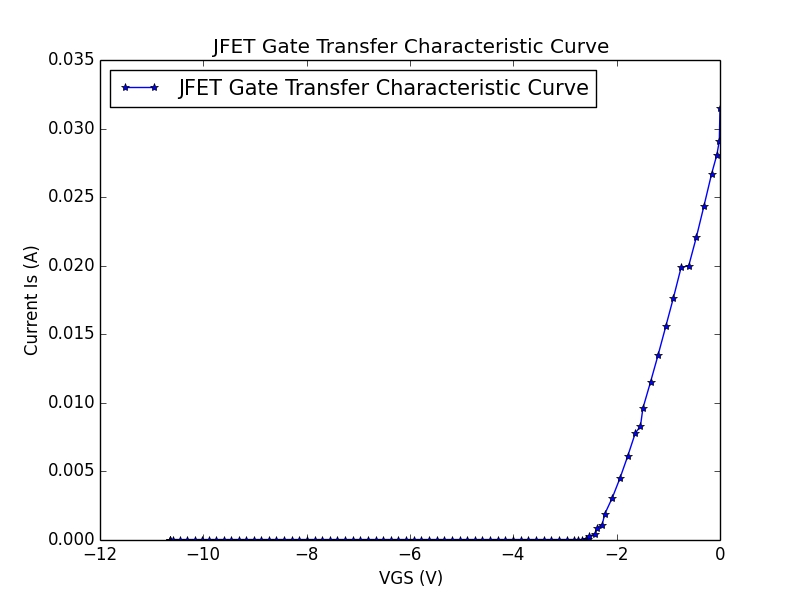
\includegraphics[scale = 0.5]{4_5.png}
        \caption{JFET Characteristic Transfer Curve}
        \label{fig:my_label}
    \end{figure}
    \begin{figure}[H]
        \centering
        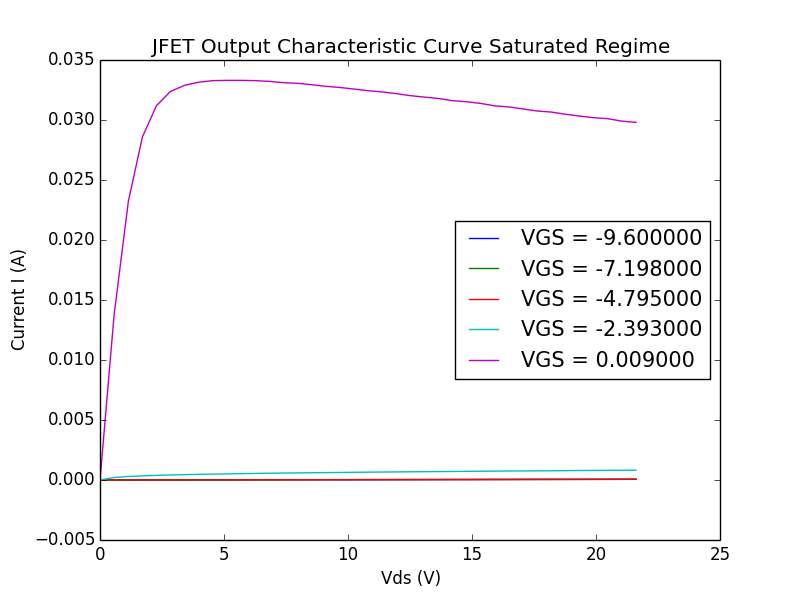
\includegraphics[scale = 0.5]{4_5sat.png}
        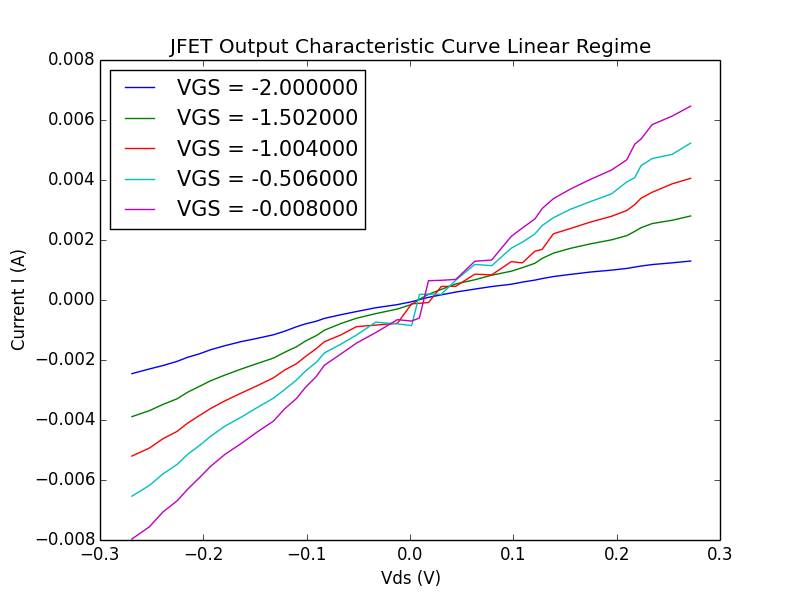
\includegraphics[scale = 0.5]{4_5lin.png}
        \caption{Saturated and linear regimes for JFET Output Characteristic Curve}
        \label{fig:my_label}
    \end{figure}
    \begin{figure}[H]
        \centering
        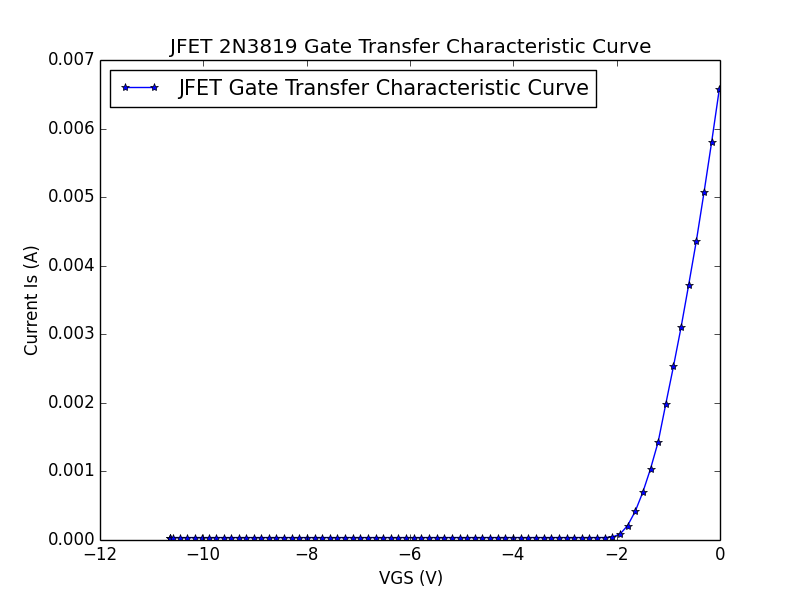
\includegraphics[scale = 0.5]{4_6.png}
        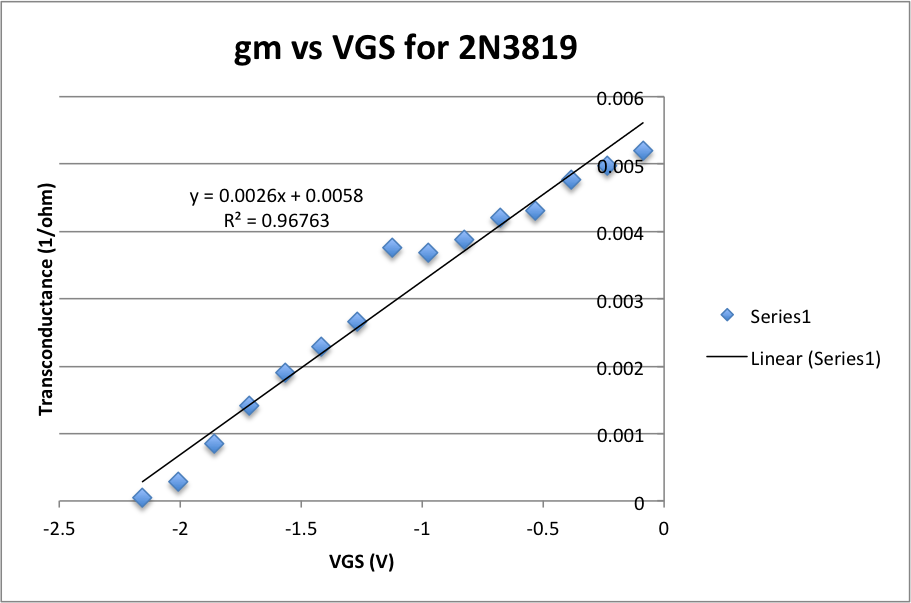
\includegraphics[scale = 0.65]{4_6b.png}
        \caption{JFET Transfer Curve and Transconductance vs $V_{GS}$ for Transistor 2N3819}
        \label{fig:my_label}
    \end{figure}
    \begin{figure}[H]
        \centering
        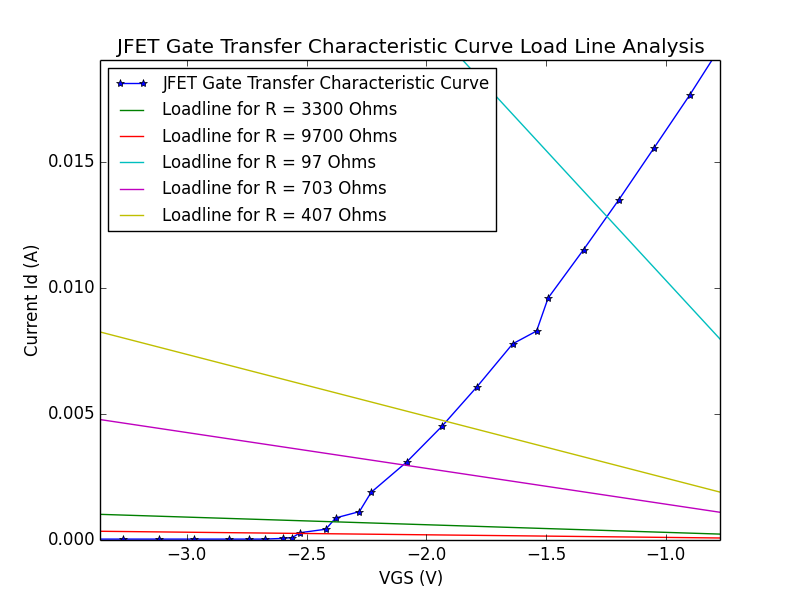
\includegraphics[scale = 0.65]{4_9.png}
        \caption{Load Line Analysis for Adjustable Self-Biased Current Source}
        \label{fig:my_label}
    \end{figure}
    \begin{figure}[H]
        \centering
        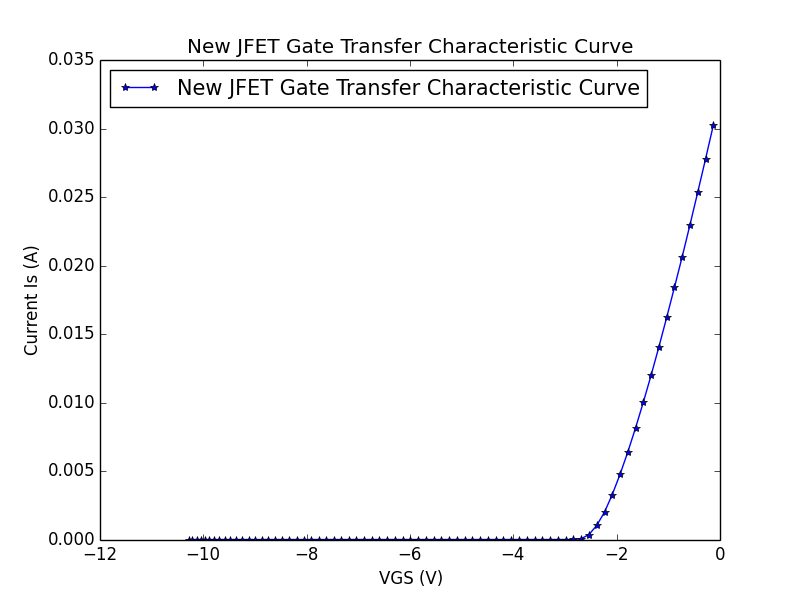
\includegraphics[scale = 0.5]{4_10a.png}
        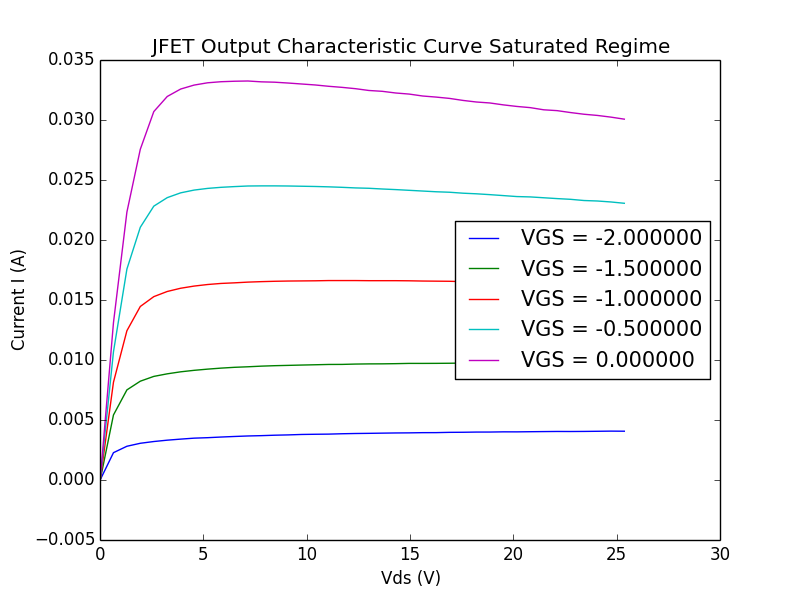
\includegraphics[scale = 0.5]{4_10b.png}
        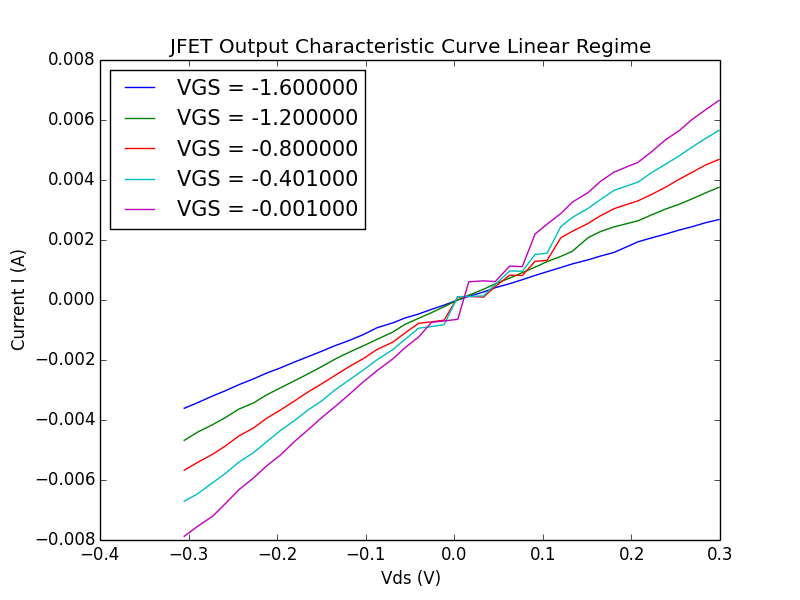
\includegraphics[scale = 0.5]{4_10c.png}
        \caption{New JFET Characteristic Curves (Transfer, saturated output, linear output)}
        \label{fig:my_label}
    \end{figure}
    \begin{figure}[H]
        \centering
        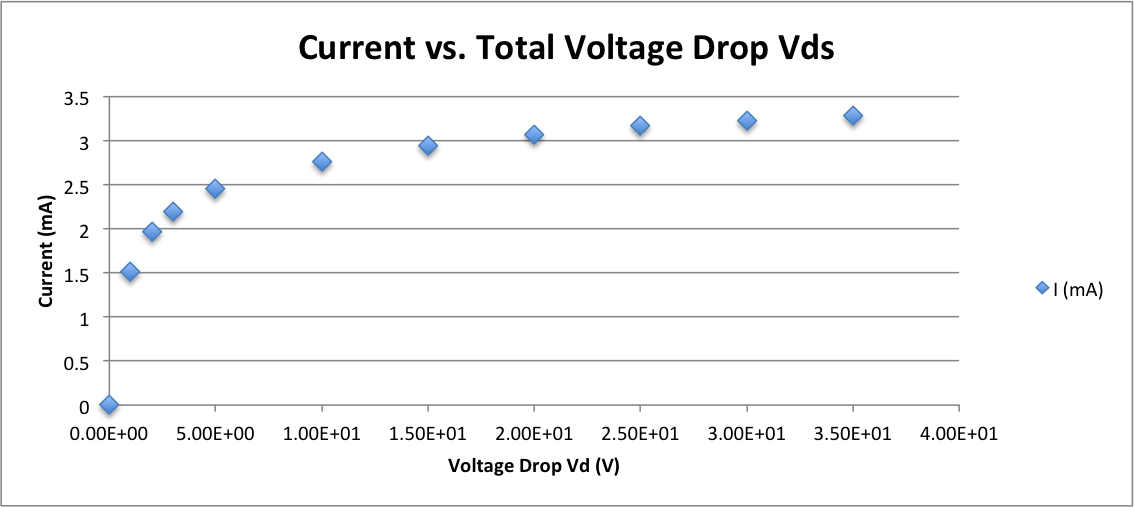
\includegraphics[scale = 0.7]{4_10d.png}
        \caption{Current vs. Total Voltage Drop for externally biased current source}
        \label{fig:my_label}
    \end{figure}
    \begin{figure}[H]
        \centering
        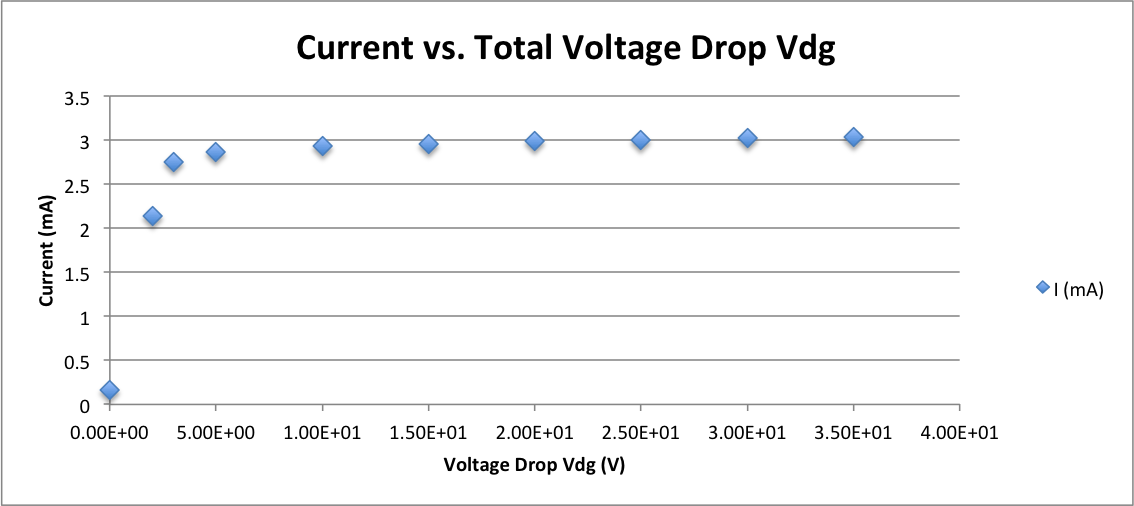
\includegraphics[scale = 0.7]{4_11.png}
        \caption{Current vs. Total Voltage Drop for self-biased current source}
        \label{fig:my_label}
    \end{figure}
\subsection{Tables}
    \begin{table}[H]
    \centering
    \caption{Data points (found in 4.4) added to JFET Transfer Curve}
    \label{my-label}
    \begin{tabular}{cc}
    \textbf{$V_{GS}$(V)} & \textbf{$I_D$ (A)} \\ \hline
    -2.74E+00 & 0.0000017 \\
    -2.60E+00 & 0.000025 \\
    -2.42E+00 & 0.000428 \\
    -2.56E+00 & 0.000096 \\
    -2.28E+00 & 0.001126 \\
    -1.54E+00 & 0.0083 \\
    -6.00E-02 & 0.02 \\
    0.00E+00 & 0.0281
    \end{tabular}
    \end{table}
    \begin{table}[H]
        \centering
        \caption{Output Current for Given Resistances (Load Line Analysis Included)}
        \label{my-label}
        \begin{tabular}{ccccc}
        \textbf{Vin = 15V} & \textbf{} & \textbf{} & \textbf{} & \textbf{} \\
        \textbf{$R_{theo}$ ($\Omega$)} & \textbf{$R_{meas}$ ($\Omega$)} & \textbf{$I_{meas}$ (A)} & \textbf{$I_{pred}$ (A)} & \textbf{Relative Error ($\%$)} \\ \hline
        100 & 97 & 0.0128 & 0.01284 & 0.31152648 \\
        390 & 407 & 0.0047 & 0.00471 & 0.212314225 \\
        703 & 703 & 0.00297 & 0.002982 & 0.402414487 \\
        3300 & 3300 & 0.000743 & 0.000732 & 1.50273224 \\
        10000 & 9700 & 0.000275 & 0.000261 & 5.363984674
        \end{tabular}
    \end{table}
    \begin{table}[H]
        \centering
        \caption{Current vs. Total Voltage Drop $V_{ds}$ for externally biased current source}
        \label{my-label}
        \begin{tabular}{cc}
        \textbf{$V_{ds}$ (V)} & \textbf{I (mA)} \\ \hline
        0.00E+00 & 0 \\
        1.00E+00 & 1.51 \\
        2.00E+00 & 1.97 \\
        3.00E+00 & 2.19 \\
        5.00E+00 & 2.46 \\
        1.00E+01 & 2.76 \\
        1.50E+01 & 2.94 \\
        2.00E+01 & 3.07 \\
        2.50E+01 & 3.17 \\
        3.00E+01 & 3.23 \\
        3.50E+01 & 3.29
        \end{tabular}
    \end{table}
    \begin{table}[H]
    \centering
    \caption{Measuring Currents Across 5 Random JFETs}
    \label{my-label}
    \begin{tabular}{cc}
    \textbf{JFET} & \textbf{Current $I_d$ (mA)} \\ \hline
    original & 5.43 \\
    1 & 6.61 \\
    2 & 4.79 \\
    {\color[HTML]{FE0000} \textbf{3}} & {\color[HTML]{FE0000} \textbf{5.49}} \\
    4 & 6.39  \\
    5 & 5.94
    \end{tabular}
    \end{table}
    \begin{table}[H]
        \centering
        \caption{Improved Follower: Input and Output Signals, and Gain for Various Input Signals}
        \label{my-label}
        \begin{tabular}{ccccc}
        \textbf{$V_{in}$ (mV)} & \textbf{f (Hz)} & \textbf{$V_{out}$ (mV)} & \textbf{$\Delta$V = $V_{out} - V_{in}$ (mV)} & \textbf{Gain} \\ \hline
        402 & 200 & 401.3 & -0.7 & 0.998258706 \\
        405.5 & 1000 & 402.5 & -3 & 0.992601726 \\
        404 & 10000 & 401.7 & -2.3 & 0.994306931 \\
        203.8 & 200 & 200 & -3.8 & 0.981354269 \\
        100.7 & 200 & 96 & -4.7 & 0.953326713 \\
        506.1 & 200 & 500 & -6.1 & 0.987947046
        \end{tabular}
    \end{table}
    \begin{table}[H]
        \centering
        \caption{Current vs. Total Voltage Drop $V_{ds}$ for self-biased current source}
        \label{my-label}
        \begin{tabular}{ll}
        \textbf{$V_{dg}$ (V)} & \textbf{I (mA)} \\ \hline
        0.00E+00 & 0.166 \\
        2.00E+00 & 2.14 \\
        3.00E+00 & 2.75 \\
        5.00E+00 & 2.87 \\
        1.00E+01 & 2.93 \\
        1.50E+01 & 2.96 \\
        2.00E+01 & 2.987 \\
        2.50E+01 & 3 \\
        3.00E+01 & 3.02 \\
        3.50E+01 & 3.03
        \end{tabular}
    \end{table}
    \begin{table}[H]
        \centering
        \caption{Finding Predicted Gain for Each Input Voltage}
        \label{my-label}
        \begin{tabular}{cccc}
        \textbf{$V_{in}$ (V)} & \textbf{$r_s$ ($\Omega$)} & \textbf{$G_{predicted}$} & \textbf{Relative Error (\%)} \\ \hline
        0.402 & 116 & 0.99942 & 0.116 \\
        0.4055 & 116 & 0.99942 & 0.682 \\
        0.404 & 116 & 0.99942 & 0.512 \\
        0.2038 & 116 & 0.99942 & 1.808 \\
        0.1007 & 116 & 0.99942 & 4.612 \\
        0.5061 & 116 & 0.99942 & 1.15
        \end{tabular}
    \end{table}


\section{Signature Page}
\centering
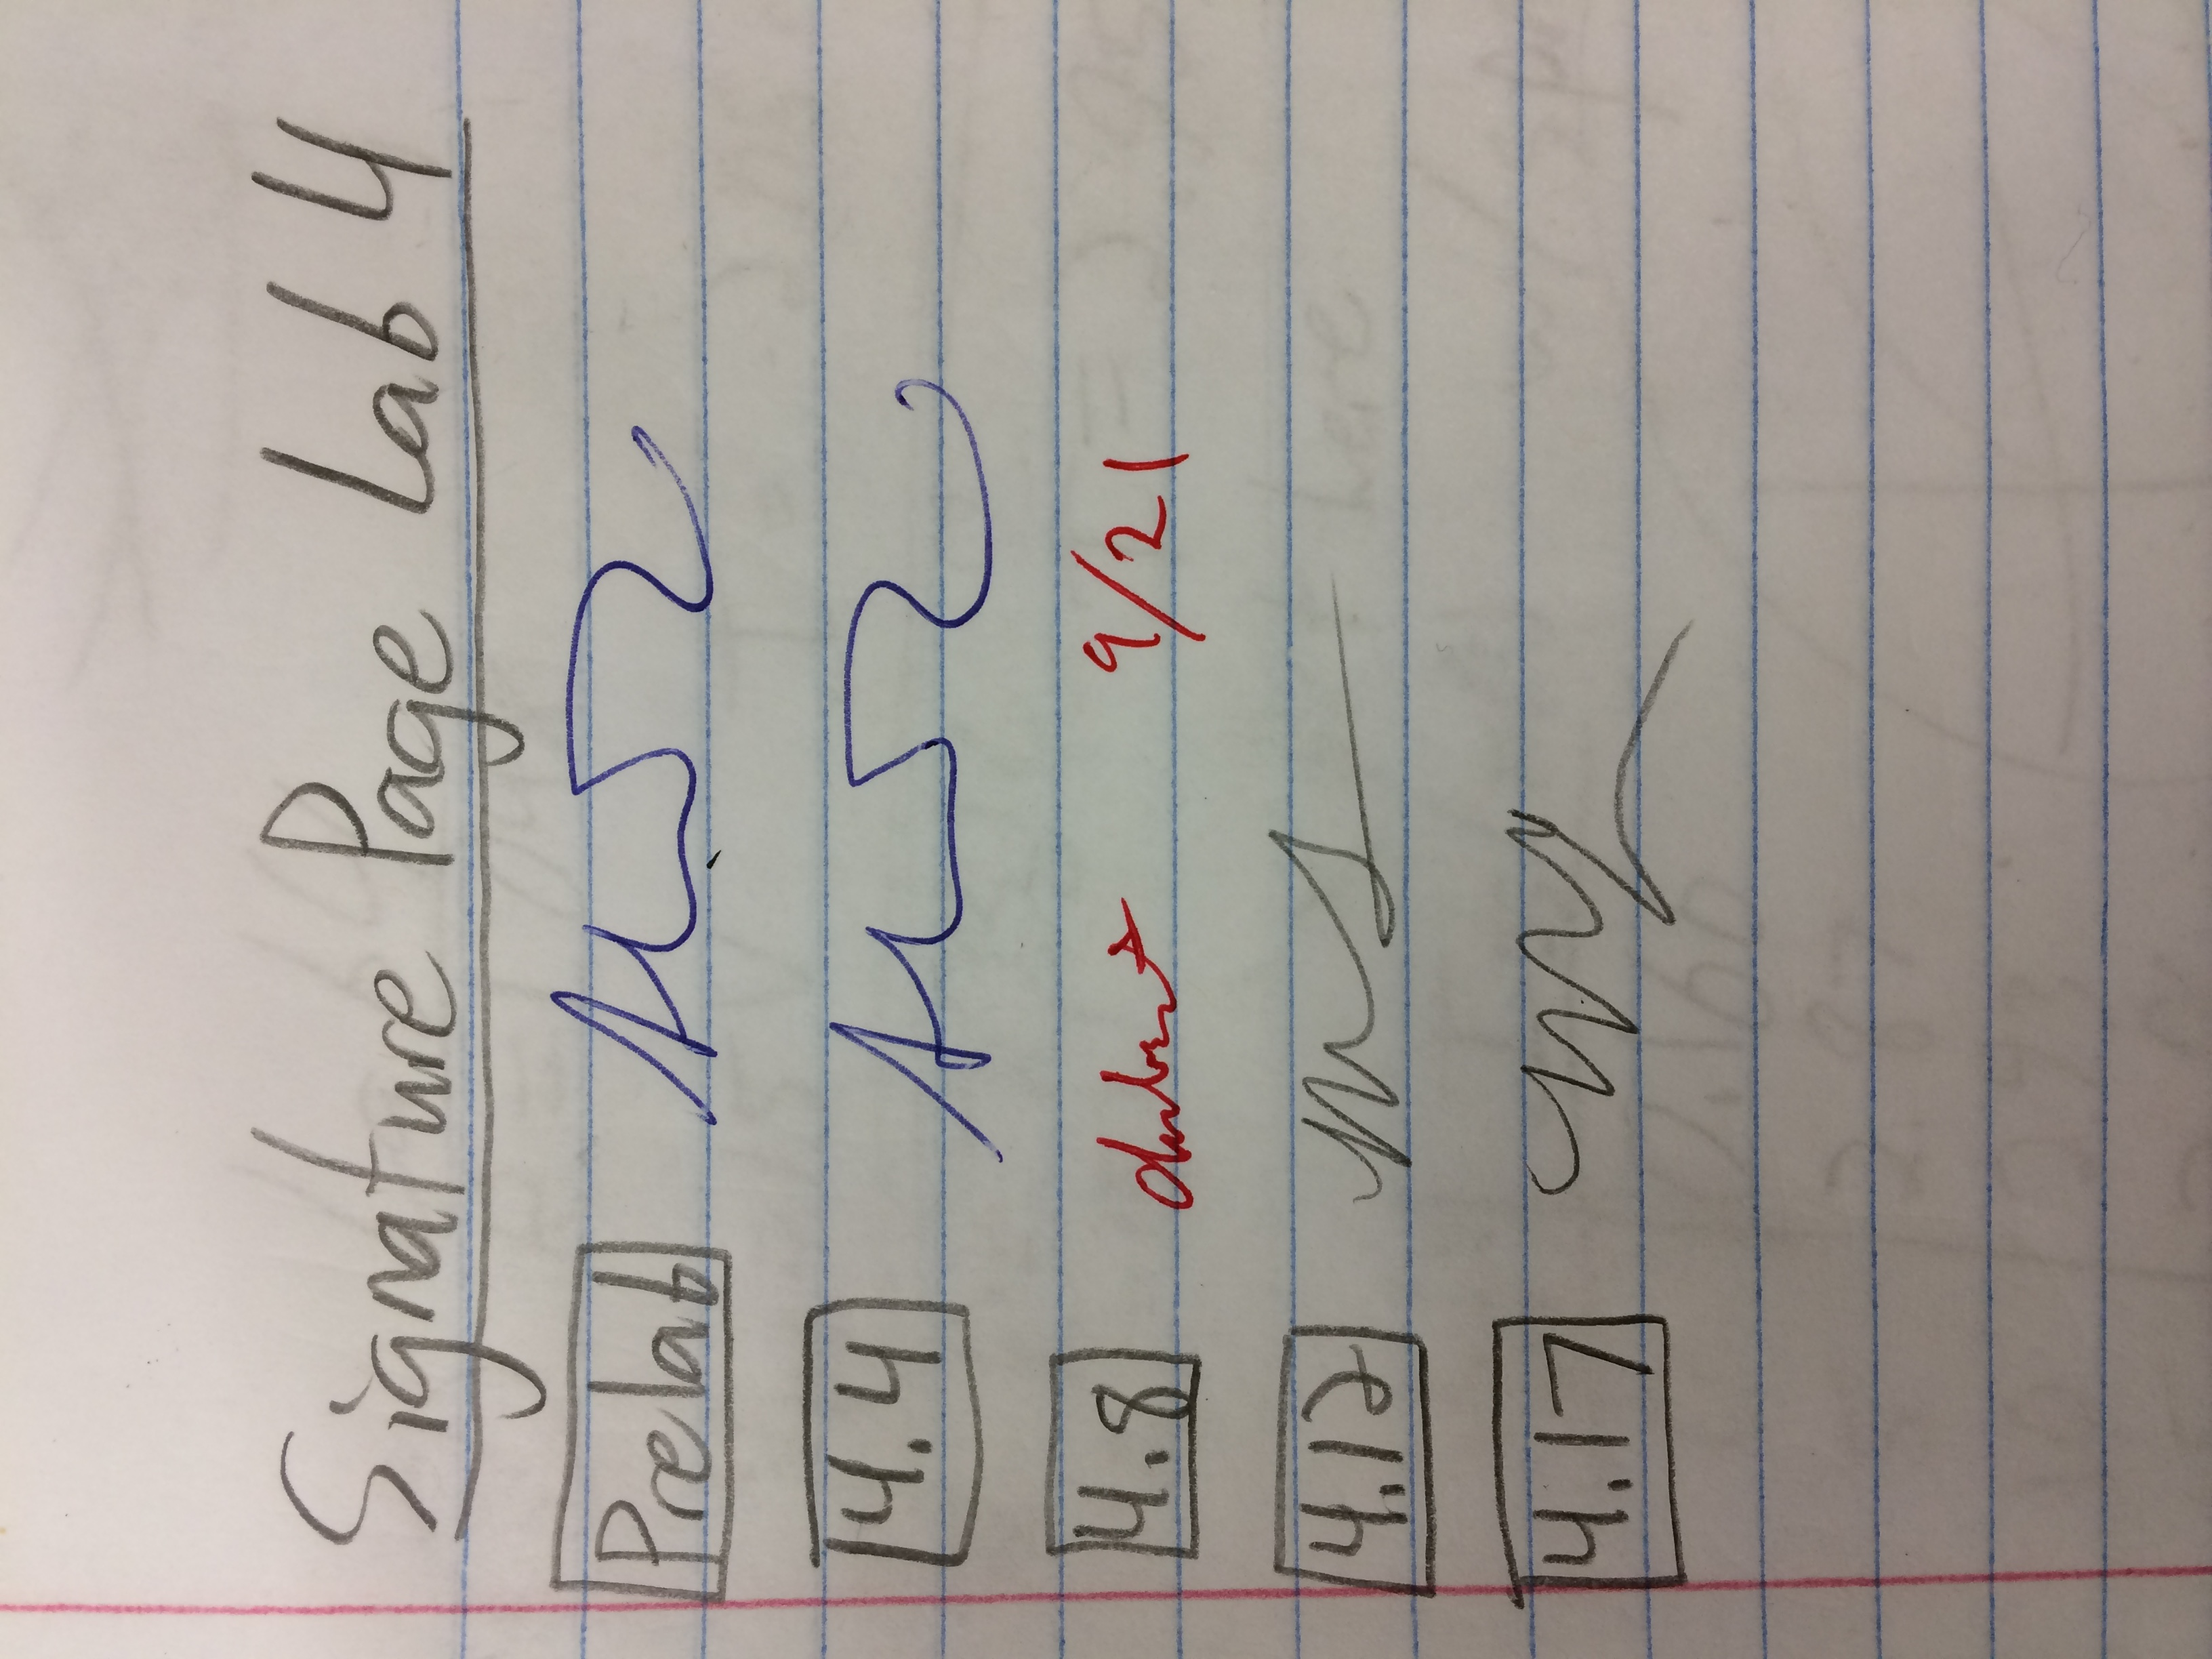
\includegraphics[scale = 0.1,angle = -90]{IMG_1154.jpeg}


\end{document}
